\documentclass[conference]{sig-alt-gov2}
\pdfpagewidth=8.5in
\pdfpageheight=11in
%\usepackage{subfig}
\usepackage{subfigure}
\usepackage[pdftex]{}
\usepackage{todonotes}
\usepackage{listings}
\lstset {% general command to set parameter(s)
         language=C,
     basicstyle=\footnotesize,               % print whole listing small
%     keywordstyle=\color{black}\bfseries, % underlined bold black keywords
%     identifierstyle =\color{black},  % nothing happens
%     commentstyle=\color{black}\emph, % white comments
     %stringstyle=\ttfamily,          % typewriter type for strings
%     stringstyle=\color{black},       % typewriter type for strings
         tabsize=4,
         showtabs=false,
     showstringspaces=false}
%can't figure this one out for particles bandwidth
%\usepackage[caption,label]{subfig}

%\newcommand{\TITLE}{D\textsuperscript{\huge{2}}T: Doubly Distributed Transactions for High Performance and Distributed Computing}

\newcommand{\DDT}{D\textsuperscript{2}T~}
\newcommand{\DDTns}{D\textsuperscript{2}T}

\hyphenation{sub-trans-ac-tion}

% in order for balance columns to work, it has to be before begin document...
%\balancecolumns

\begin{document}

\conferenceinfo{MSST'14,} {November 17, 2013, Denver, Colorado, USA.}
\CopyrightYear{2014}
%\crdata{978-1-4503-1103-8/11/11}
\clubpenalty=10000
\widowpenalty = 10000

\title{Considerations for the Next Iteration of the DOE Fast Forward Storage and IO Project}

\numberofauthors{3}
\author{
\alignauthor Jay Lofstead\\
       \affaddr{Sandia National Laboratories}\\
       \email{gflofst@sandia.gov}
\alignauthor Ivo Jimenez\\
       \affaddr{University of California, Santa Cruz}\\
       \email{ivo@cs.ucsc.edu}
\alignauthor Carlos Maltzahn\\
       \affaddr{University of California, Santa Cruz}\\
       \email{carlosm@soe.ucsc.edu}
%\and  % use '\and' if you need 'another row' of author names
}
\maketitle

\begin{abstract}
The Fast Forward effort to define a next generation filesystem has made
admirable contributions in architecture and design. Formalizing the general
idea of data staging as burst buffers for the file system will help manage
the performance variability and offer the data processing opportunities
outside the main compute and file system. Adding a tranasctional mechanism to
manage faults and data visilibilty helping to enable effective analytics
without having to work around the IO stack semantics.

While these and other contributions are valuable, improvements can be
incorporated. For example, the Doubly Distributed Transactions (\DDTns)
protocol offers an alternative approach for incorporating transactional
semantics into the data path. The differing semantics between the two
approaches and the functionality provided offer alternatives. Further, the
lessons learned in implementing \DDT has generated insights into what the
FastForward file system could and perhaps should do, given different features.

This paper examines some of the choices made by the FastForward team and
compares them with other options and offers suggestions based on experiences.

\end{abstract}

\category{D.4}{Software}{Operating Systems}
\category{D.4.7}{Operating Systems}{Organization and Design}[hierarchical design]

\terms{Design, Performance}

\section{Introduction}

Current production HPC IO stack design is unlikely to offer sufficient features
and performance to adequately serve the needs of an extreme scale platform. To
address these limitations, the US Department of Energy commissioned an effort
to develop a design and prototype for an IO stack suitable for the extreme
scale environment. This is a joint effort led by the Intel Lustre team, Los
Alamos National Laboratory, EMC, and the HDF Group. This team has developed a
specification for a future IO stack to address the identified challenges.

The basic architecture incorporates five layers. The top layer is a high level
IO library, such as the demonstration HDF-5 library. Below that is an IO
forwarding layer that redirects IO calls from the compute nodes to the IO
dispatching layer. This IO forwarding layer is analogous to the function of the
IO nodes in a BlueGene machine. The IO dispatcher (IOD) has considerable
functionality.

The IOD serves as the sole interface between an application and the persistent
storage array. The core idea for IOD is to provide a way to manage the IO load
that is separate from the compute nodes and the storage array. Communication
intensive acitivies, such as two-phase, data sieving IO's data rearrangement
phase, can be moved to the IOD layer offloading the communication load from the
compute nodes. IOD has three main purposes. First, if the optional burst
buffer is availble, it works as a fast cache absorbing write write operations
for the slower trickle out to the central storage array. It can also be used to
retrieve objects from the central storage array for more efficient read
operations. Second, it offers the transaction mechanism for controlling data
set visibility prior to it being correct and complete. Third, data processing
operations can be placed in the IOD. This operations are inteded to offer data
rearrangement, filtering, and similar operations prior to it reaching the
central storage array.

This offloads the requirement for collective two-phase data sieving
on the compute nodes to reorganize data. This technique has been proven
effective at reducing the total time for writing data due to fewer participants
involved in the communication patterns~\cite{lofstead:2011:nessie-staging}.

The bottom two layers are the Data Access Object Storage (DAOS) and Virtual
Object Storage Device (VOSD). DAOS is the typical interface that represents
the individual objects stored including the semantics related to ``files''.
VSOD is the actual storage mechanism for the objects defined at the DAOS layer.

Incorporated into the design of these layers and the function of some of these
layers themsleves, such as the IOD layer, are features to manage both burst IO
performance and faults. In particular, the IOD layer's use of burst buffers
attempts to absorb a massive data dump from the compute area that is then trickled to the persistent storage area only if desired. Otherwise, it can be stored
locally on optional SSDs for use by analysis routines eliminating the need to
use slower rotational media as the intermediary between a simulation and the
analysis code.

A second feature is the incorporation of a transaction like mechanism into the
IOD layer and a related epochs feature into the DAOS layer. This feature offers
a mechanism to avoid making incomplete data visible to other users and offer a
level of protection if the data can be stored on the optional SSDs.

These features aim to address both the bursty nature of HPC IO and to make the
data storage stack resilient to faults. While these features can address these
concerns, a deeper evaluation of the design suggests exploring alternatives
may improve the performance and/or functionality desired.

The rest of the paper is organized as follows. Section~\ref{sec:burst}
discusses some of the features of incoporating burst buffers as designed and
suggests some considerations and alternatives for the next generation of this
project. Section~\ref{sec:transactions} discusses the transactions approach
offered in the IOD layer and offers a comparison to the \DDT system.
Section~\ref{sec:optimizations} discusses some of the optimizations offered
by the current design and how and when these optimizations will work best. It
also explores some of the dark corners that may yield performance issues with
the current design. Finally, Section~\ref{sec:summary} disucsses the system
overall with recommendations on what design elements should be reconsidered
based on broader issues with current HPC data centers.

\section{Burst Buffers}
\label{sec:burst}

The idea of burst buffers were initially explored in the context of data
staging~\cite{abbasi:2007:datatap,Abbasi:2009:datatap,nisar:2008:staging,zheng:2010:predata}
and later incorporated as part of the IO
stack~\cite{bent:2012:challenges,bent:2012:burst-buffer}. The proposed optional
use of SSDs is problematic. First, with these burst buffers being optional, the
semantics of how IOD works must change to use DAOS to store the data directly
rather than storing them locally until explicitly persisted by the user. How
this work work, the impact on metadata, and the ability to support
functionality such as data reordering, such as chainging the fast dimension of
an array, is undefined. How doing function shipping into an IOD without a burst
buffer would work is also not explored. Further thought about how to have an
IOD layer both with and without a burst buffer is required before they can be
considered optional. As the design stands today, they are a required part of
the IOD layer for proper functioning.

\section{Transactions and Epochs}
\label{sec:transactions}

The transaction mechanism manifests in two forms. At the IOD layer, they are
called transactions and are used to judge whether or not an output is complete
or not. At the DAOS layer, they are called epochs and represent persisted
transactions from the IOD layer. Each of these offers different functionality,
but are connected as is explained below.

\subsection{IOD Transactions}
To understand how transactions are used in the IOD layer, some terminology and
concepts must be explained first. At the coarsest grain level is a container.
Each container serves to host a transaction and contains a collection of
objects. Conceptually, containers corresponds to a file in a traditional file
system. The objects in each container represent different data within a file.
The three initially defined object types are key-value store, array shard,
and blob. The easiest way to understand these types is to evaluate these from
the perspective of an HDF-5 file. The key-value store represents a collection
of attributes. The array shard represents part of a potentially
multi-dimensional array. It is refered to as a shard because it is likely a
small piece of a globally defined array. The blob represents a byte stream.
The fundamental difference between an array shard and a blob is that the array
shard has metadata identifying its portion within the global, logical space
while the blob is simply a 1-dimensional array of bytes that is not shared
across IOD nodes. Should an operation be deployed into IOD to manipulate an
array within a container, it would operate on the array shards rather than on
blobs. Given this context, the transactions come in two forms.

First is a single leader transaction where the IOD manages based on calls from
a single client. The underlying assumption is that the client side will manage
the transactional operations itself and the single client is capable of
reporting to the IOD how to evolve the transaction state. 

The second form is called multi-leader and has the IOD layer manage the
transactions. In this case, when the transaction is created, a count of clients
is provided to the IOD layer. As clients write to the container, the reference
count is reduced. Once the count reaches 0, the transaction is automatically
committed.

\subsection{DAOS Epochs}
The Epoch mechanism differs from transactions. Instead of focusing on when a
particular output is complete, an epoch represents incremental persisted copies
of a container. Each persisted copy increments the epoch. NEED TO CORRECT
THIS INFORMATION AS IT IS WRONG.

\subsection{Metadata Management}
While a central design goal of IOD and DAOS is to eliminate the metadata server
as a core component, it was not fully accomplished.  The purpose behind the goal
is to eliminate the serialized bottleneck caused by having a centralized
metadata service. Much of the design of IOD with objects and continers does
work to eliminate these bottlenecks. However, IOD does not go fully to a no
metadata service model. Instead, the IOD layer describes a key-value metadata
service it provides. This service maintains four different items:

\begin{itemize}
\item The list of IOD objects within the container
\item The mapping from each IOD object to the corresponding DAOS object.
\item The sharding and striping of the IOD object
\item The maximum valid offset of the object
\end{itemize}

While a pure no metadata model would be ideal for performance, this current
proposal has a few challenges. First, there are no list of containers. This
is closer to the no metadata ideal, but given the rest of the functionality,
it exports to the user level a requirement to track what containers are in the
file system. Second, given the flattening that occurs between IOD and DAOS,
the mapping from IOD objects to DAOS objects is not likely to be 1-to-1. This
is likely a list instead. Further, given the ability to re-stripe in the IOD
layer, the list is not a list of objects completely included in the IOD object,
but instead objects from which part of the data came from some listed DAOS
object.  Third, sharding IOD objects makes sense based on the compute process
connection a shard has with the complete object. Striping of an IOD object
makes sense in connection with the DAOS object(s) underneath, but striping
within the IOD layer is not discussed. Further, using striping from clients
into the IOD layer introduces a level of coordination that IOD seeks to avoid.
Fourth, given the previous items, there is ambiguity with the maximum valid
offset of the object. This could be for the shard or for the collection of
shard objects that represent a distributed variable.

The \DDT project created a simplistic model for a metadata service that has
different features that is described below and has been published about
previously~\cite{lofstead:2012:txn-metadata}. Some of the major differences
include the following. First, \DDTns's metadata service has a way to get a list
of the ojbjects in the metadata service. While it does not address having a
file equivalence like the container concept, it does introduce a way to figure
out what is available. Stored along with this object description is a list of
the global dimensions for array objects. One observtion made as part of
creating this service is that this is insufficient for many engineering codes
that use non-regular meshes. Second, for each object, a list of the equivalent
to shards are kept with a link back to the master object and the offset and
size for each dimension for that shard. This approach is not scalable because
of the explosion in the process count. Using a striping approach like IOD does
is superior. Third, there is no mapping to another layer with different object
layout and counts.

Based on the lessons from the \DDT metadata service construction, having a
completely separate metadata service is workable. Rather than making it a
bottleneck in the IO path, it is another service that users must interact with
if they need those services. Otherwise, it is 100% out of the way. Users can
manage everything by maintaining the metadata including the list of objects
themselves. However, there are drawbacks to this 100% client-side approach.

For the IOD proposal, the service needs some adjustments to be generally
useful.  First, there needs to be a way to query the list of available
containers. Second, the maximum transaction ID for a container is mentioned as
being maintained by this metadata service, but when and how this is done is
never mentioned. Second, it should be extracted from IOD entirely and kept as
a separate service along side. This will eliminate any contention caused by
interaction with the IOD layer. This also offers a way to link with the DAOS
layer in a machine-independent way. The need for this is described below.
Third, the definition of an object needs to be made more clear. In some cases,
it seems that an object is a globally distributed object is represented by a
collection of shards. In other cases, it is a single shard.

\subsection{Comparison to \DDTns}
The \DDT project~\cite{lofstead:2012:txn} sought to develop an efficient
approach for handling ACID-style transactions in an environment with parallel
clients and multiple servers (doubly distributed). Rather than being aimed
solely at data movement operations, \DDT seeks to address the general problem
of managing any operation with multiple clients and servers.  Consider the
management of the analysis/visualization area, potentially similar to the IOD
concept. The transaction protocol is used to help manage resizing of the
resource allocation to the various analysis and visualization components.  For
the purposes of this discussion, \DDT could also be used to manage changing how
IOD processes and/or nodes are used without exposing these changes to the
client processes prematurely.  This has been described and analyzed
previously~\cite{dayal:2013:io-containers}.

To address the gap between pure \DDT and IOD's transactions, example data
storage and metadata services were created. These examples were not built for
performance but to determine the minimum functionality requirement for a
functional service. While these services were built without knowledge of how
IOD and DAOS operate, we came to similar functionality. The major difference is
that there are no dependencies between transactions that prevent visibility
should an older version be incomplete. This additional, intentional requirement
by IOD offers different functionality than \DDTns's example services. In the
case of \DDTns, the functionality is more minimal, but also avoids some of the
concerns outlined below.

The second iteration of the protocol~\cite{lofstead:2013:pdsw-txn} fixed
scalability issues and demonstrated a scalable client-side coordiation model
with excellent performance. The performance measured for a complex transaction
with \DDT is illustrated in Figure~\ref{fig:performance}. This performance is
explored in detail in a previous paper~\cite{lofstead:2013:pdsw-txn}. The
breakdown of the number of participants in each role is shown in
Table~\ref{tab:scaling}. For comparison, consider the Number of
Sub-Coordinators equivalent to an IOD process. The Processes Per
Sub-Coordinator represents the number of clients that use a particular IOD. For
these tests, we maintained a balanced distribution and always used at least two
sub-coordinators to slow down the processing.

\begin{figure}[ht]
%\vspace{-0.15in}
\centering
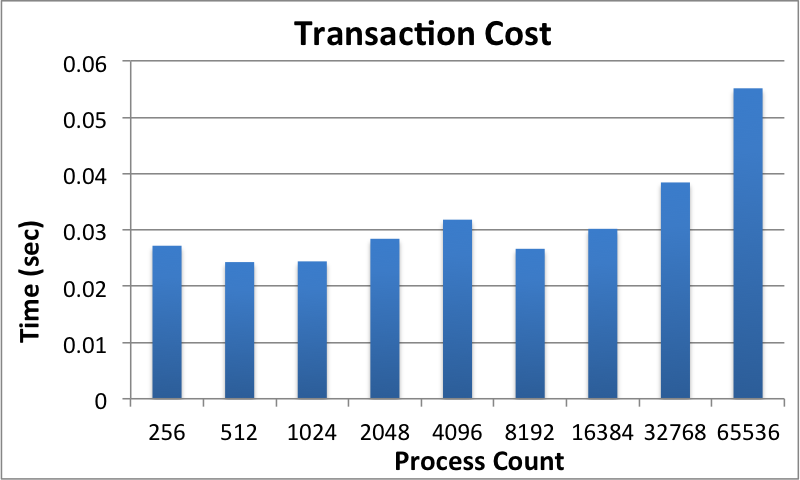
\includegraphics[keepaspectratio=true, width=0.9\columnwidth]{images/performance}
\vspace{-0.15in}
\caption{Total Transaction Overhead}
\label{fig:performance}
\vspace{-0.15in}
\end{figure}

\begin{table}[ht]
    \vspace{-0.15in}
    \centering
    \caption[Scaling Configuration]{Performance Tests Scaling Configuration}
    \bigskip
    \vspace{-0.15in}

    \begin{tabular}{|r|r|r|}
\hline
Processes & \vtop{\hbox{\strut Number of}\hbox{\strut Sub-Coordinators}} & \vtop{\hbox{\strut Processes Per} \hbox{\strut Sub-Coordinator}}\\
\hline
%8 & 2 & 4 \\
%16 & 2 & 8 \\
%32 & 2 & 16 \\
%64 & 2 & 32 \\
%128 & 2 & 64 \\
256 & 2 & 128 \\
512 & 2 & 256 \\
1024 & 4 & 256 \\
2048 & 8 & 256 \\
4096 & 16 & 256 \\
8192 & 32 & 256 \\
16384 & 64 & 256 \\
32768 & 128 & 256 \\
65536 & 256 & 256 \\
\hline
    \end{tabular}
    \label{tab:scaling}
\end{table}

At a a high level, both \DDT and the IOD transactions have the same high-level
design. In both cases, a hierarchical model is employed. In the case of \DDTns,
it is a purely client-side tree. For IOD, it is a server-side tree. In both
cases, there is a master in charge of managing the transaction and a collection
of workers that aggregate into the master through second-level leaders. Beyond
that, there are some significant differences. Some of the different choices
made by IOD raise some possible concern.

First, \DDT has a timeout mechanism to detect failures and offer an ability to
recover and clean up the incomplete transactions. IOD's transactions are
asynchronous precluding a relatively simple, short timeout value to detect
failures. Unfortunately, at this point, there is no mechanism in IOD's
transaction handling to detect a fault and clean up any incomplete operations.

Second, should a transaction on a container not complete, all subsequent
transactions on that container, even if they are complete and correct, will not
be accessible.

Third, in the single leader model, if the process that manages the transaction
were to fail, there is no ability to abort that transaction. The data will not
be made available because the transaction is still listed as in progress. The
problem is that without a way to clean up this failed transaction, no newer
versions of the same container can be made readable. In reality, the single
leader model would ideally outsource the transaction processing to something
like \DDT on the client side.

Fourth, in the multi-leader model, using a count of client connections to
determine if transaction is complete is problematic.  First, should this be in
an evnironment where lost or repeated network messages are possible, then the
count could be wrong inappropriately. This is a general problem and unlikely
in the current environment, but is a concern on less integrated platforms.
The idea of a count precludes any tracking of expected messages from sources
introducing a potential hole. Second, the aggregation of completion messages
are based on the local aggregation point reporting to the transaction
leader the state.  There is no ability to detect or recover from a failure of
this IOD process that would report to the transaction leader. Third, because a
simple count of participating processes is sent with the beginning of the
transaction, each process is strictly limited to a single output operation.
This precludes a process writing multiple array shards, for example. To put
this in concrete terms, it means that a file could only contain a single,
globally distributed variable (at the root level of HDF5) OR an attribute per
process. If this count actually represents a begin/end transaction pair
instead, it suffers from a lack of accountability for missing object (shard)
writes. All it would indicate is that a process started and ended a transaction
connection.

\begin{figure}[ht]
\centering
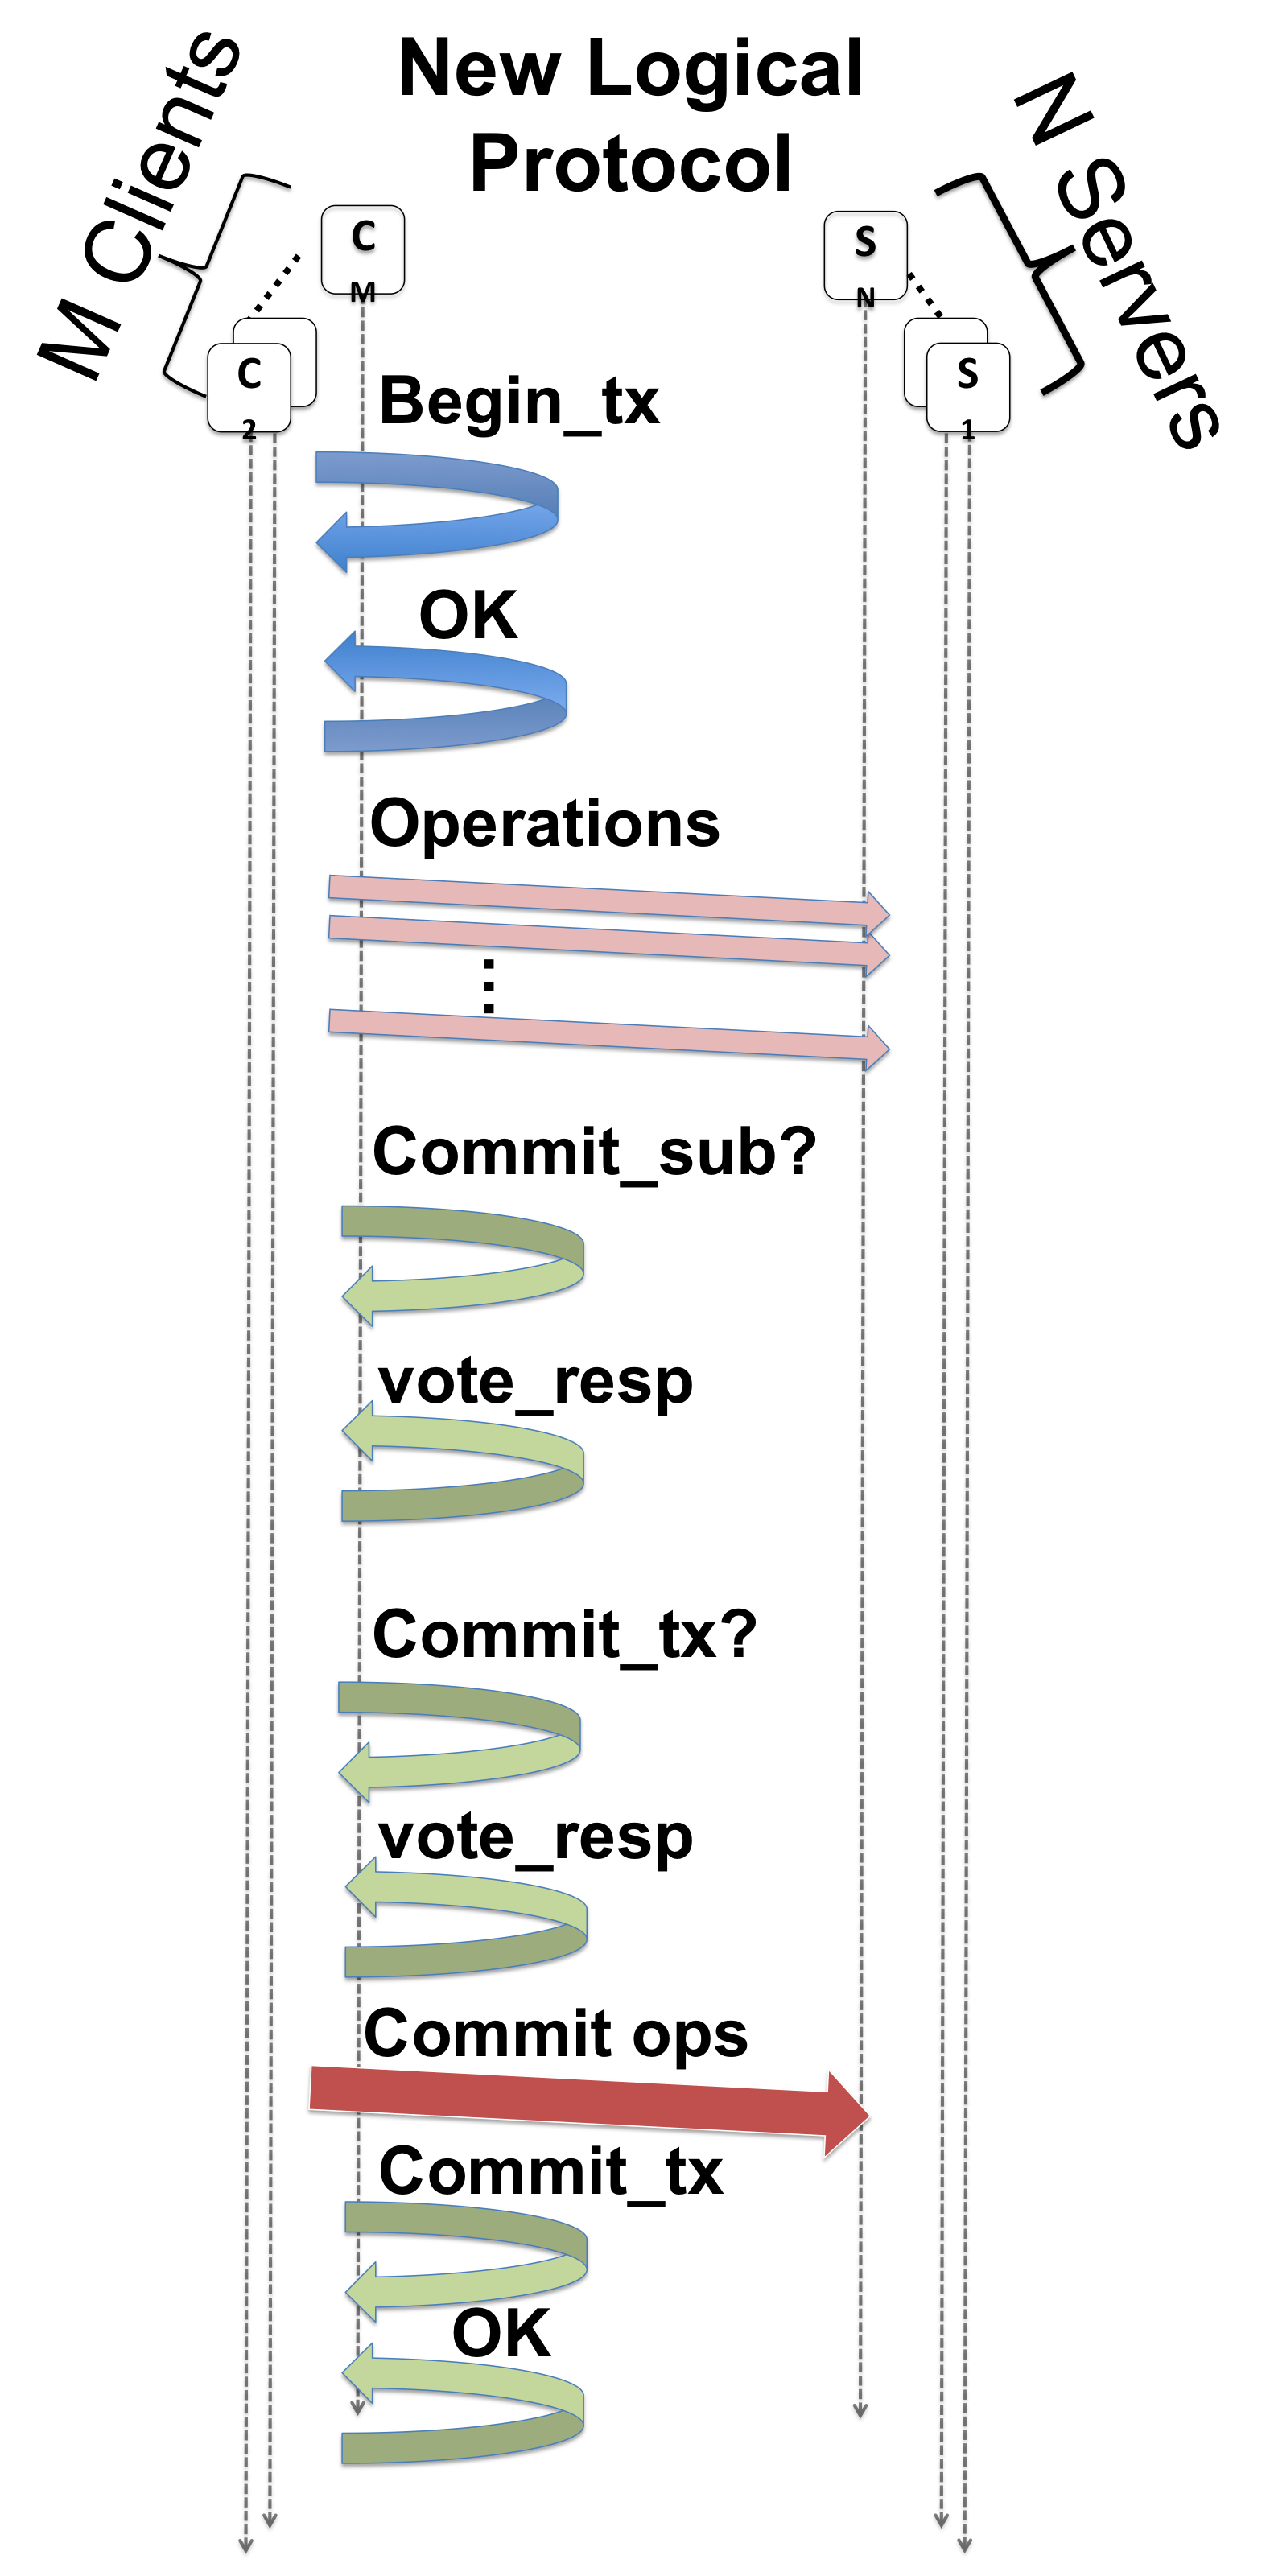
\includegraphics[keepaspectratio=true, width=0.9\columnwidth]{images/optimized-protocol}
\vspace{-0.15in}
\caption{Optimized Protocol}
\label{fig:optimized-protocol}
\vspace{-0.25in}
\end{figure}

\DDT has addressed this count issue in a couple of ways. First, the
sub-coordinators each have a list of processes from which they expect messages.
Should a message be missed, it is noticed and corrective action can be taken.
Second, \DDT has the concept of sub-transactions. The messaging requirements
are illustrated in Figure~\ref{fig:optimized-protocol}.  Sub-transactions
represent finer grained operations than the entire output, \DDT can manage
multiple writes per client by using a sub-transaction to represent the output
for any item to the file (container). Because of how the sub-transactions are
managed, the singleton sub-transactions must be declared before the transaction
begins ensuring there is global knowledge that the sub-transaction is expected.
That way if the coordinator (transaction leader) fails, which ever process
takes over that role knows to expect a completion message for that
sub-transaction or the overall transaction cannot complete. While this
additional layer does introduce messaging, the overhead is quite small.

\subsection{Comparision to Other Protocols}
Alternatives, such as Paxos~\cite{Lamport:1998:paxos} algorithms like
ZooKeeper~\cite{Hunt:2010:zookeeper}, suffer from two limitations making them
unsuitable for this environment. First, the distributed servers in Paxos
systems are all distributed copies of each other that eventually become
consistent. Given the scale we wish to address, a single node's memory is
unlikely to be able to hold all of the data necessary for many operations at
scale. They also do not have a guaranteed for when consensus will be
achieved without using slower synchronous calls. For the tight timing we wish
to support, we need guarantees of when a consistent state has been achieved.
Second, these systems also all assume that updates are initiated from a single
client process rather than a parallel set of processes as is the standard in
HPC environments. The Intel/Lustre FastForward epoch
approach~\cite{barton:2013:fastforward,lombardi:2013:epochs} is discussed in
Section~\ref{lab:evaluation}.

Third, the server must offer a way to mark an operation as ``committed'' during
the ``commit'' phase of the two-phase commit.  Again, this may be implemented
in a transactional wrapper.  As an alternative, a scalable locking service like
Chubby~\cite{burrows:2006:chubby} might be employed.

Fourth, a second layer of coordination on the client side is introduced that
greatly increases the scalability by consolidating messages from clients into
unique sets prior to sending to the overall coordinator. A gossip
protocol~\cite{ganesh:2003:gossip-protocols} may appear sufficient for this
purpose, but the delay of eventual consistency is strictly avoided with this
protocol to ensure guarantees at particular states in the code. For example, if
a failure occurs, the global understanding of the role of all processes is
required in order for effective communication to occur for operations like
creating sub-transactions or voting. In this case, the protocol can offer
stronger statements about consistency than these protocols offer.  These
features offer a way to easily scale the transaction protocol given the
guarantees we wish to offer.

Another effort to offer consistency and data integrity for the ZFS file
system~\cite{zhang:2010:zfs} covers some of the same territory. Instead of a
focus on the processes all having a notion of completion as a transaction, this
work focuses on the integrity of the data movement operations. We view this
work as something that should be considered hand-in-hand with a transaction
approach to ensure the integrity of the movement of the data in addition to the
agreement of processes about the successful completion of a parallel operation.

\section{Optimizations}
\label{sec:optimizations}

The ability to place functionality at the IOD layer was explored earlier. In
particular, PreDatA~\cite{zheng:2010:predata} demonstrated the advantage to
the approach as well as identified that the placement of the operators should
consider the compute nodes, the staging or burst buffer nodes, or offline
depending on the characteristics of the operation. This consideration should
be incorporated into the design. In particular, one of the key observations
is that the reduced process count may require the entire time between output
operations to perform many of the data processing tasks requested. This was
part of the motivation prompting evaluating placement decisions at the compute
node, in a staging area, or offline. In the case of the IOD design, it forces
a staging area deployment and then shares that staging area across all users
simultaneously. This is unlikely to be useful because of the limited compute
and communication capacity to spare to perform these operations at a bottleneck
in the IO path. The use of a separate staging area to perform these computations
intentionally selects a location separate from the IO path to avoid these
bottlenecks and potential scalability issues.

\section{Broader Design}
\label{sec:summary}

Consider a shared file system across an HPC data center. The current design
maintains the metadata in the IOD layer localized to a single machine
effectively making the data inaccessible from another platform.

There is a change in definitions between the IOD layer and the DAOS layer.
For the IOD layer, a container is a collection of objects. For the DAOS layer,
a continer is a collection of shards. For the IOD an object may be a shard of
a global array. For DAOS, a shard can host a set of DAOS objects. Having the
same names with locally correct, globally conflicting definitions serves to
confuse how the system should work.

\section{Conclusions}
\label{lab:conclusion}

We have demonstrated that synchronous two-phase commit transactions can have
low overhead and be used with roughly synchronous operations with little
additional overhead. While other use cases, particularly those that require a
greater degree of asynchrony, require a different approach, \DDT offers a
working solution for a wide variety of scenarios today.  The bigger question of
what sort of synchronization mechanism is appropriate for various use cases is
currently under investigation.

The evaluation of the fault detection and recovery are beyond scope for this
paper and are in preparation for presentation elsewhere.

\section{Acknowledgements}

\includegraphics[scale=0.07]{logos/doe_logo}

\includegraphics[scale=0.30]{logos/snl_logo}

\includegraphics[scale=0.35]{logos/nnsa_logo}
Sandia National Laboratories is a multi-program laboratory managed and operated
by Sandia Corporation, a wholly owned subsidiary of Lockheed Martin
Corporation, for the U.S. Department of Energy's National Nuclear Security
Administration under contract DE-AC04-94AL85000.

\bibliographystyle{abbrv}
\bibliography{paper}

\vfill\eject

\newpage
%%%%%%%%%%%%%%%%%%%%%%%%%%%%%%%%%%%%%%%%%%%%%%%%%%%%%%%%%%%%%%%%%%%%%%%%%%%%%%%

%\begin{figure}[ht]
%\vspace{-0.15in}
%\centering
%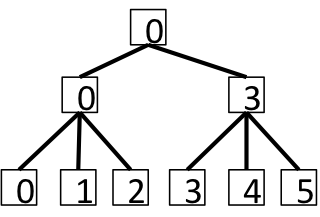
\includegraphics[keepaspectratio=true, width=0.9\columnwidth]{images/hierarchy}
%\vspace{-0.15in}
%\caption{Example Hierarchy}
%\label{fig:hierarchy}
%\vspace{-0.15in}
%\end{figure}

%\begin{figure}[ht]
%\centering
%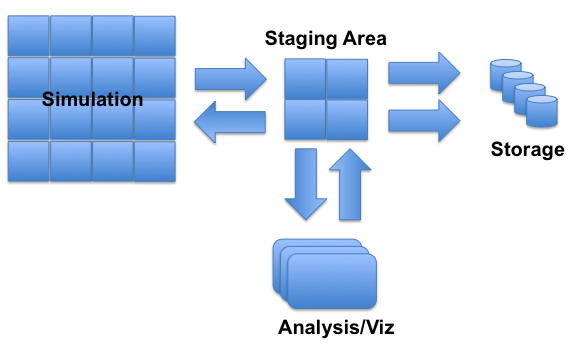
\includegraphics[keepaspectratio=true, width=0.9\columnwidth]{images/stagingmodel}
%\vspace{-0.15in}
%\caption{Staging Model}
%\label{fig:staging-model}
%\vspace{-0.15in}
%\end{figure}

%\section{New Protocol Design}
%\label{lab:design}

%To summarize the semantics of \DDT for those unfamiliar with it, consider the
%following. Since we have parallel clients and servers (MxN), it is necessary to
%have a mechanism to manage each single operation by a collection of clients 
%with a collection of servers to ensure that it is completed correctly. We must
%also have a way to manage the set of these operations as a single, atomic
%action. The difficulty with this scenario is the need to maintain global
%knowledge across all of the clients and servers. This global knowledge allows
%decisions across all clients. In a traditional distributed transaction, the
%single client always knows the state reported by all of the ``server''
%resources used. When the client is split into multiple pieces, each piece
%ultimately needs to have the same knowledge, including any knowledge that might
%be local only. If this does not happen, no guarantees can be made. The message
%count explosion implied by this level of knowledge is daunting and what
%prompted this project. Adding complexity for data movement operations is that
%a typical data set will contain multiple globally distributed variables that
%each must be treated as an atomic unit.

%To accommodate these requirements, we have the concept of a transaction
%representing the total set of operations and the sub-transaction representing a
%single operation. Each sub-transaction can represent either a single process
%performing an action (singleton) or all of the parallel clients participating
%in a single action (global). In either case, each sub-transaction is managed as
%part of the overall transaction. Voting and commit operations are performed
%both at the sub-transaction level and at the transaction level. With the
%re-implementation of the protocol, these semantics have not changed.

%\section{Evaluation}
%\label{lab:evaluation}

%To evaluate the scalability and performance of \DDTns, tests are performed on
%Cielo at Sandia National Laboratories. Cielo is a Cray XE6 platform with 8,944
%nodes each containing dual, eight core AMD Opteron 6136 processors and 32 GB of
%RAM. It uses the Cray Gemini network in a 3D torus and uses the Cray Linux
%Environment. Tests are performed at powers of two scale from 256 up to 65536
%processes. We use two pairs of datastore and metadata services along side the
%process counts mentioned here. Each of these other services is given a single
%node on which to operate.

%The represented IAW consists of a writing application creating ten 3-D
%variables. Each of these variables is distributed across all of the processes
%with each process containing a 32x32x32 double precision floating point number
%chunk for each variable. The total space is scaled by doubling each dimension
%keeping the total dimensions as close to square as is possible. All ten of
%these variables and the corresponding chunks are written to the first pair of
%datastore and metadata servers. Then, an update application marks one variable
%as ``in process'' in the first metadata service, reads the chunks in parallel
%from the first datastore service, updates the data, creates a new variable in a
%second metadata service inserting the updated data into the second datastore
%service, and then deletes the original variable from the first datastore and
%metadata services. For the purposes of this evaluation, only the overhead
%incurred by the transaction protocol is reported.  No attempts were made to
%make the datastore and metadata service efficient and including those
%performance results would obfuscate the impact of having transactions surround
%data movement applications. The overheads are measured during the update
%application's activities and represent the green and blue arrows within
%Figure~\ref{fig:optimized-protocol}.

%With the three-tier structure employed by \DDTns, we choose to always employ at
%least two sub-coordinators, even at small scale, to incur higher overhead
%costs.  An example of this configuration is shown in
%Figure~\ref{fig:hierarchy}.  In this case, process 0 acts as the coordinator,
%sub-coordinator, and a subordinate. Process 3 acts as a sub-coordinator and a
%subordinate. The rest of the processes operate solely as subordinates. The
%configuration for each run consists of a minimum of 2 sub-coordinators and a
%maximum of 256 subordinates per sub-coordinator. That yields 256
%sub-coordinators each with 256 subordinates at 65536 processes. This is
%illustrated in Table~\ref{tab:scaling} showing the various scales evaluated and
%the configuration for each.  Other tests of smaller numbers of processes were
%run, but were omitted because they did not add any additional information to
%the results.

%The test values reported include the following actions:

%\begin{enumerate}
%\item txn\_create\_transaction - create a new transaction
%\item txn\_create\_sub\_transaction - create a new singleton sub-transaction
%\item txn\_create\_sub\_transaction\_all - called three times to create three global sub-transactions
%\item txn\_begin\_transaction - start the transaction processing
%\item txn\_commit\_sub\_transaction - called four times total to commit the four sub-transactions
%\item txn\_vote\_transaction - vote to commit or abort the overall transaction
%\item txn\_commit\_transaction - commit the entire transaction
%\item txn\_finalize\_txn - clean up any transaction specific memory or perform any final operations
%\end{enumerate}

%All operations except txn\_create\_sub\_transaction and \\
%txn\_commit\_sub\_transaction are performed as effectively collective
%operations. These two exceptions are only performed by the single process
%involved. In order for the existence of this singleton sub-transaction to be
%guaranteed to be known, we split the create and begin operations to provide a
%timeframe during which all singleton sub-transactions should be initialized.
%The begin operation gathers knowledge of all of these singleton
%sub-transactions and broadcasts it to all processes to make failure recovery
%possible. This step guarantees that every singleton sub-transaction will be
%known or the begin will fail due to a process failure. Since the global
%sub-transactions are global operations, they can be done either before or after
%the begin transaction call. In our case, we have one global sub-transaction
%created before the begin transaction and two afterwards.

%The selected sequence of operations gives a representative idea of what a
%typical transaction may include. Each test is performed seven times and the
%mean value is presented. Given the small magnitude of the values, there is a
%bit of variance that has a large percentage, but small absolute value. The
%results are presented in Figure~\ref{fig:performance}. The results for 4096
%processes were lost.

%In the interest of saving space, only the results for 64K processes is
%discussed. In all cases, the time spent in operations for the 64K case are the
%longest of all cases tested. At a detailed level, the time for the 64K
%processes case can be itemized as follows. First, the slowest operation, by
%far, is the txn\_create\_sub\_transaction\_all with a maximum time of 0.0310
%seconds for one of the calls. The mean time is 0.01 seconds. Second, the other
%operations are all at less than 0.005 seconds on average and a maximum of 0.012
%seconds.  Third, the time for the initialization and cleanup of the total
%protocol, the calls equivalent to MPI\_Init and MPI\_Finalize, take 0.38
%seconds total. Since the txn\_init call is the first call that uses MPI in the
%system and that it is a full order of magnitude slower than any other operation
%at worst, we believe there is MPI initial communication channel setup being
%established accounting for the extra time. The txn\_finalize takes a maximum of
%0.0002 seconds.  Since these calls are done once for the entire application
%lifetime, we did not include them in the results since they are not part of the
%typical transaction cost that would be incurred for each transactional
%operation.

%\section {Discussion}
%\label{lab:discussion}
%The leading alternative to \DDT is the Intel/Lustre FastForward Epoch
%approach~\cite{barton:2013:fastforward,lombardi:2013:epochs}.  While \DDT is
%intended for a general purposes, epochs are designed specifically to address
%the needs of a shared storage array with a large number of parallel clients.
%The general idea is to mark every operation with a transaction id, record a
%process count somewhere to allow reconciliation later, and have every process
%operate independently for the duration of the writing operation. A second, more
%synchronous mode is also available. In this synchronous mode, the user is
%required to manage the transaction ID and to update the transaction state in
%the storage servers. During a read process, it must be determined what is the
%most current, complete, ``Readable'' version of the file.  This entails
%contacting all of the storage devices to determine all of the versions of
%blocks stored on each device. With that information, it can be determined which
%of these transactions is ``Readable''. While this reconciliation operation may
%happen asynchronously, it must be done before a read operation potentially
%prompting it to be triggered by a client call or potentially stale data is
%presented as the most current.

\end{document}
